\documentclass[problem]{mcs}

\begin{pcomments}
  \pcomment{CP_triangle_tiling_recursive}
  \pcomment{sequel to CP_triangle_tiling}
  \pcomment{S16.cp5m}
  \pcomment{ARM 2/26/16}
\end{pcomments}

\pkeywords{
 induction
 DET
 triangle
}


%%%%%%%%%%%%%%%%%%%%%%%%%%%%%%%%%%%%%%%%%%%%%%%%%%%%%%%%%%%%%%%%%%%%%
% Problem starts here
%%%%%%%%%%%%%%%%%%%%%%%%%%%%%%%%%%%%%%%%%%%%%%%%%%%%%%%%%%%%%%%%%%%%%

\begin{problem}
Divided Equilateral Triangles (DETs) were defined in
\inbook{problem~\bref{CP_triangle_tiling}}\inhandout{an earlier class
  problem~\bref{CP_triangle_tiling}} as follows:

\begin{itemize}

\item \textbf{Base case:} A single equilateral triangle is a
  DET whose only subtriangle is itself.

\item If $T \eqdef$ 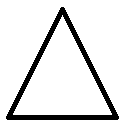
\includegraphics[width=1cm]{tiling_1} is a DET,
  then the equilateral triangle $T'$ built out of four copies of $T$
  as shown in in Figure~\ref{4DETrec-fig} is also a DET, and the
  subtriangles of $T'$ are exactly the subtriangles of each of the
  copies of $T$.
\end{itemize}
Properties of DETs were proved earlier by induction on the length of a
side of the triangle.  Recognizing that the definition of DETs is
recursive, we can instead prove properties of DETs by structural
induction.

\begin{center}
\begin{figure}\inbook{[h]}
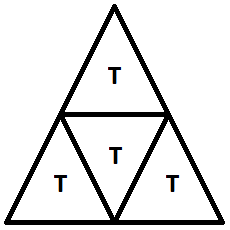
\includegraphics[width=2cm]{tiling_2}
\caption{DET $T'$ from Four Copies of DET $T$}
\label{4DETrec-fig}
\end{figure}
\end{center}

\bparts

\ppart\label{DETcorner} Prove by structural induction that a DET with one of its corner
subtriangles removed can be tiled with trapezoids built out of three
subtriangles as in Figure~\ref{3traprec-fig}.

\begin{center}
\begin{figure}\inbook{[h]}
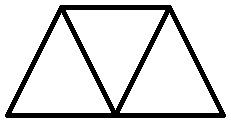
\includegraphics[width=2cm]{tiling_3}
\caption{Trapezoid from Three Triangles}
\label{3traprec-fig}
\end{figure}
\end{center}

\begin{solution}
The structural induction hypothesis is that if a DET, $T'$, has one of
its corner subtriangles removed, then it can be trapezoid-tiled.

\inductioncase{Base case} ($T'$ is a single equilateral triange): Here
the only corner subtriangle is $T'$ itself, and removing the corner
leaves nothing, which can be tiled with no trapezoids.  This proves
the base case.

\inductioncase{StructuralInduction step} ($T'$ consists of
four copies of some DET $T$ as in Figure~\ref{4DETrec-fig}.)

Without loss of generality, we assume that the top corner subtriangle
of $T'$ is removed.  This removed triangle is also the top corner of
copy 1 of $T$ as shown in Figure~\ref{traptilerec-fig}.

By structural induction hypothesis, each copy of $T$ with a corner
triangle removed can be trapezoid-tiled.  So copy 1 of $T$ with the
top triangle removed can be trapezoid-tiled.  Also if we remove the
right corner of copy 2 of $T$, the bottom corner of the inverted copy
3, and the left corner of copy 4, what remains of copies 2--4 can each
be trapezoid-tiled.  The hole left by the middle 3 missing corners at
the bottom of $T'$ can then be tiled with a single trapezoid, yielding
a complete tiling by trapezoids of $T'$ with its top corner removed.

\begin{center}
\begin{figure}\inbook{[h]}
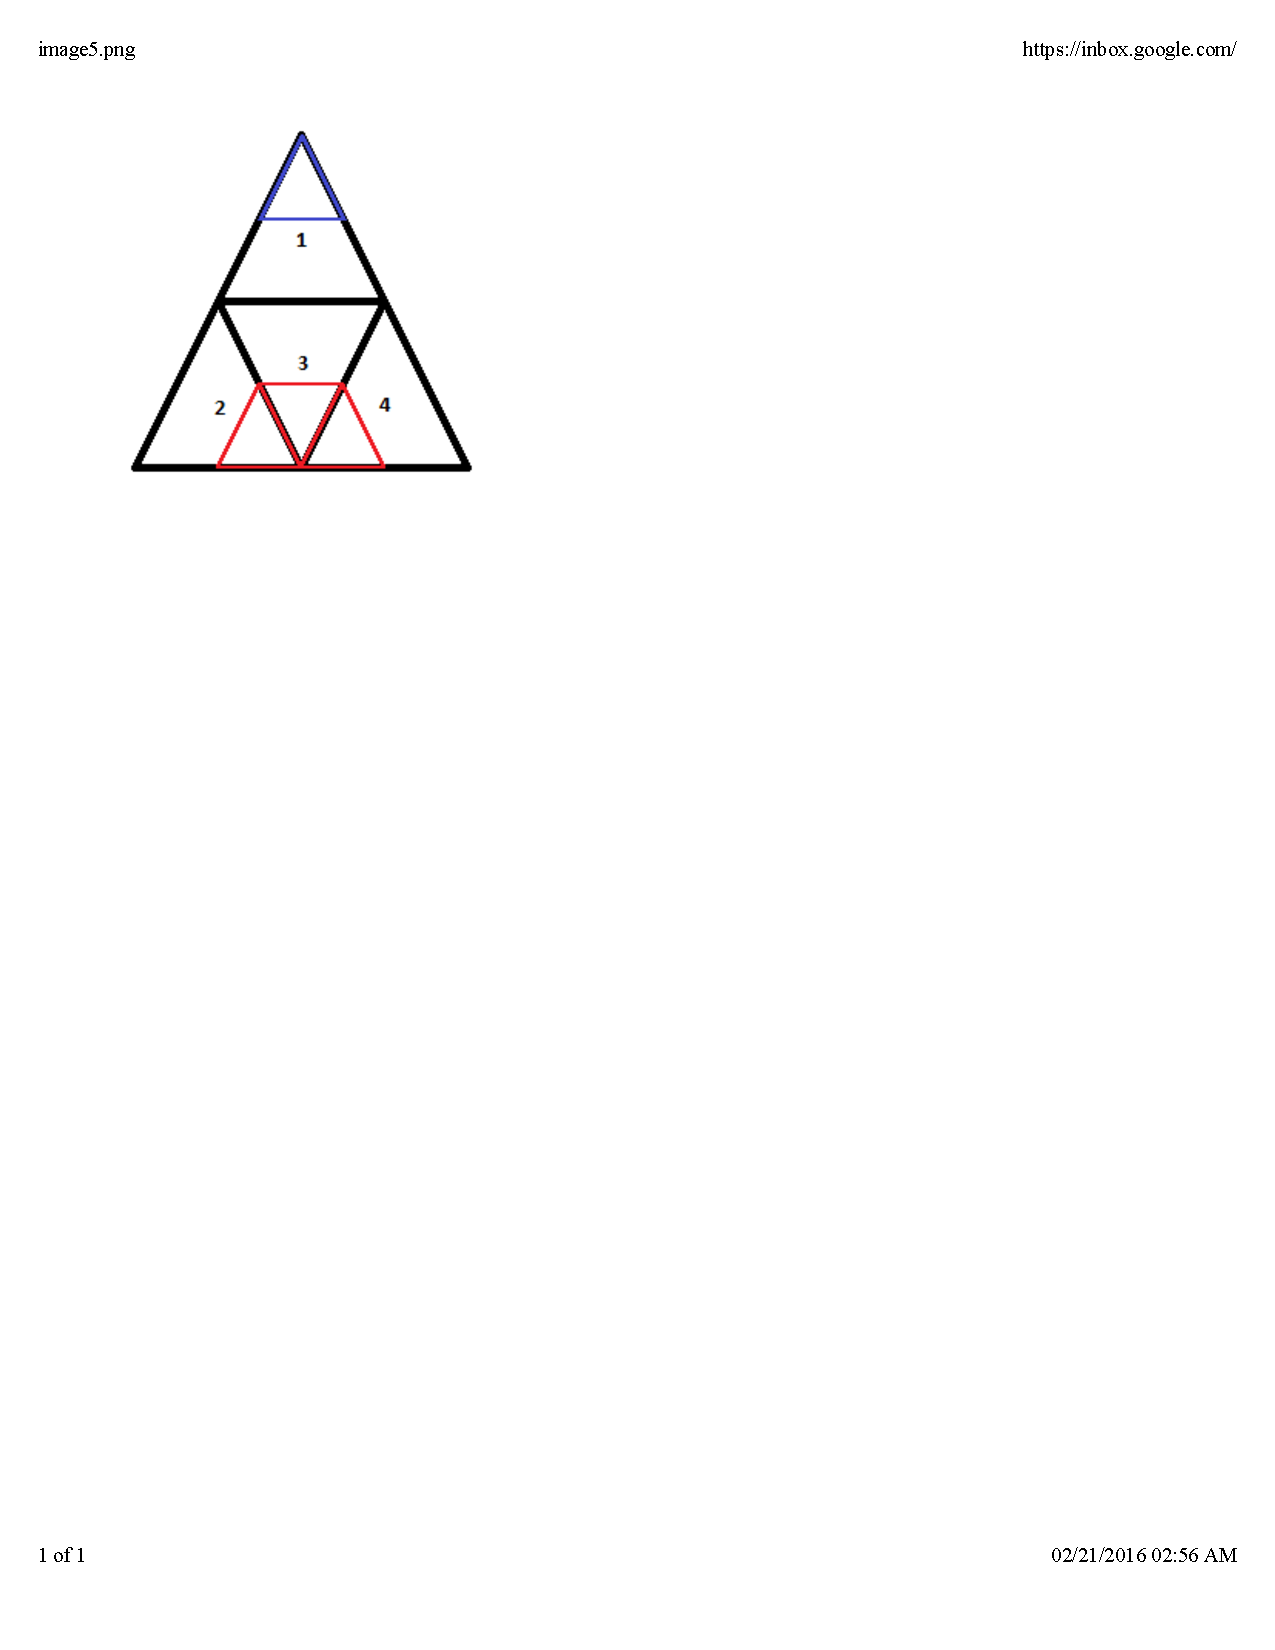
\includegraphics[width=3cm]{tiling_5}
\caption{Tiling $T'$ with trapezoids}
\label{traptilerec-fig}
\end{figure}
\end{center}

We conclude by structural induction that any DET with a corner removed
can be trapezoid-tiled.
\end{solution}

\ppart\label{removemiddle} Explain why a DET with a triangle removed from the middle of
one side can also be tiled by trapezoids.

\begin{solution}
Referring again to Figure~\ref{traptilerec-fig}, note that the lower left
triangle of copy 1 of $T$ is a middle triangle of $T'$.  With this
triangle removed, copy 1 of $T$ can be trapezoid-tiled by
part~\eqref{DETcorner}, and the rest of $T'$ can be tiled as in
part~\eqref{DETcorner}.
\end{solution}

\ppart In tiling a large square using L-shaped blocks as described in
\inbook{Section~\bref{subsec:tile_induction}}\inhandout{the text},
there was a tiling with any single subsquare removed.
Part~\eqref{removemiddle} indicates that trapezoid-tilings are
possible for DETs with a non-corner subtriangle removed, so it's
natural to make the mistaken guess that DETs have a corresponding
property:
\begin{falseclm*}
A DET with any single subtriangle removed can be trapezoid-tiled.
\end{falseclm*}

We can try to prove the claim by structural induction as in
part~\eqref{DETcorner}.

\begin{bogusproof}
The claim holds vacuously in the base case of a DET with a single
subtriangle.

Now let $T'$ be a DET made of four copies of a DET $T$, and suppose we
remove an arbitrary subtriangle from $T'$.

The removed subtriangle must be a subtriangle of one of the copies of
$T$.  The copies are the same, so for definiteness we assume the
subtriangle was removed from copy 1.  Then by structural induction
hypothesis, copy 1 can be trapezoid-tiled, and then the other three
copies of $T$ can be trapezoid-tiled exactly as in the solution to
part\eqref{DETcorner}.  This yields a complete trapezoid-tiling of
$T'$ with the arbitrary subtriangle removed.

We conclude by structural induction that any DET with any subtriangle
removed can be trapezoid-tiled.
\end{bogusproof}
What's wrong with the proof?

\hint Find a counter-example and show where the proof breaks down.

\begin{solution}
A counter-example is a DET with just four subtriangles.  Removing the
middle triangle leaves the other three triangles without a shared
side, making a trapezoid tiling impossible.

The mistake in the proof is the remark that there is no loss of
generality in assuming the removed subtriangle came from copy 1---or
another of the corner copies of $T$.  The proof ignores the case when
the removed subtriangle is inside copy 3 in the middle of $T'$.  The
counterexample shows that the proof breaks down immediately in that
case.
\end{solution}

We don't know if there is a simple characterization of exaclty which
subtriangles can be removed to allow a trapezoid tiling.

\eparts

\end{problem}

%%%%%%%%%%%%%%%%%%%%%%%%%%%%%%%%%%%%%%%%%%%%%%%%%%%%%%%%%%%%%%%%%%%%%
% Problem ends here
%%%%%%%%%%%%%%%%%%%%%%%%%%%%%%%%%%%%%%%%%%%%%%%%%%%%%%%%%%%%%%%%%%%%%

\endinput
